
\chapter{Linear Program Estimates}
%\head \refy{9}. Linear Programming Bounds\endhead
%\heads{\refy{9}. Linear programming bounds}

% Linear Programming Stuff

%\chapter{Linear Programs} %subsection
\label{sec:linearprogram}

We have completed \shortversion{the first half}\longversion{a major
portion} of the proof of the Kepler conjecture by proving that every
contravening plane graph is tame.

The \shortversion{second half}\longversion{final portion} of the
proof of the Kepler conjecture consists in showing that tame graphs
are not contravening, except for the isomorphism class of graphs
isomorphic to $G_{fcc}$ and $G_{hcp}$ associated with the
face-centered cubic and hexagonal close packings.

This part of the proof treats all contravening tame graphs except
for three cases $G_{fcc}$, $G_{pent}$,\index{pentahedral prism} and
$G_{hcp}$. The two cases $G_{fcc}$ and $G_{hcp}$ are treated in
Theorem~\ref{lemma:local-optimality},  and the case
$G_{pent}$\index{pentahedral prism} is treated in
\shortversion{\cite{thesis}.}
\longversion{\Part~\ref{part:ferguson}.}

The primary tool that will be used is linear programming. The
linear programs are obtained as relaxations of the original
nonlinear optimization problem of maximizing $\sigma(D)$ over all
decomposition stars whose associated graph is a given tame graph
$G$.  The upper bounds obtained through relaxation are upper
bounds to the nonlinear problem.

To eliminate a tame graph, we must show that it is not
contravening. By definition, this means we must show that
$\sigma(D) < 8\,\pt$.  When a single linear program does not yield
an upper bound under $8\,\pt$, we branch into a sequence of linear
programs that collectively imply the upper bound of $8\,\pt$. This
will call for a sequence of increasingly complex linear programs.


For each of the tame plane graphs produced in
Theorem~\ref{theorem:classification}, we define a linear
programming problem whose solution dominates the value of
$\sigma(D)$ on the set of decomposition stars associated with the
plane graph. A description of the linear programs is presented in
this \chap.

\begin{theorem}\label{lemma:fcc-hcp-pent}
    %\proclaim{Theorem 9.1}
%Let $G$ be any tame plane graph.  One of the following holds.
%    \begin{enumerate}
%        \item $G$ is the plane graph of the pentahedral prism,
%         hexagonal-close packing, or face-centered cubic.
%        \item $G$ is not contravening.
%    \end{enumerate}
If the plane graph of a contravening decomposition star is
isomorphic to one in the list \cite{web}, then it is isomorphic to
one of the following three plane graphs: the plane graph of the
pentahedral prism, that of the hexagonal-close packing, or that of
the face-centered cubic packing.
%$G_{fcc}$, $G_{hcp}$, or $G_{pent}$.
\end{theorem}

This theorem is one of the central claims described in
Section~\ref{sec:logic} that lead to the proof of the Kepler
conjecture.


\section{Relaxation}

(NLP) Let $f:P\to\R$ be a function on a nonempty set $P$. Consider the
nonlinear maximization problem
    $$\max_{p\in P} f(p).$$

(LP): Consider a linear programming problem
    $$\max\, c\cdot x$$ such that $A\, x\le b$, where $A$ is a matrix,
    $b$, $c$ are vectors of real constants and $x$ is a vector of
    variables $x = (x_1,\ldots,x_n)$.  We write the linear
    programming problem as
    $$\max(c\cdot x : A\,x\le b).$$

An {\it interpretation\/} $I$ of a linear programming problem (LP)
is a nonempty set $|I|$, together with an assignment $x_i\mapsto
x_i^I$ of functions $x^I_i:|I|\to\R$ to variables $x_i$.  We say
the constraints $A\,x\le b$ of the linear program are {\it
satisfied\/} under the interpretation $I$ if for all $p\in |I|$,
we have $$A\, x^I(p) \le b.$$ The interpretation $I$ is said to be
a {\it relaxation\/} of the nonlinear program (NLP), if the
following three conditions hold.
%
 \index{interpretation}
 \index{satisfaction}
 \index{relaxation}
 \index{linear programming}
 \index{LP}
    \begin{enumerate}
    \item  $P=|I|$.
    \item The constraints are satisfied under the interpretation.
    \item $f(p)\le c\cdot x^I(p)$, for all $p\in|I|$.
    \end{enumerate}

\begin{lemma}
\label{lemma:bound} Let (LP) be a linear program with relaxation $I$ to
(NLP). Then (LP) has a feasible solution.  Moreover, if (LP) is bounded
above by a constant $M$, then $M$ is an upper bound on the function
$f:|I|\to\R$.
\end{lemma}

\begin{proof}
A feasible solution is $x_i = x_i^I(p)$, for any $p\in |I|$. The rest is
clear.
\end{proof}

\begin{remark}  In general, it is to be expected that the
interpretations $A\,x^I \le b$ will be nonlinear inequalities on
the domain $P$.  In our situation, satisfaction of the constraints
will be proved by interval arithmetic.  Thus, the construction of
an upper bound to (NLP) breaks into two tasks: to solve the linear
programs and to prove the nonlinear inequalities required to
satisfy the constraints.
\end{remark}

There are many nonlinear inequalities that enter into our
interpretation, which have been proved by interval arithmetic on
computer.  These inequalities are listed at \cite{web}.

\begin{remark}
\label{remark:derived} There is a second method of establishing the
satisfaction of inequalities under an interpretation. Suppose that we
wish to show that the inequality $e\cdot x\le b'$ is satisfied under the
interpretation $I$. Suppose that we have already established that a
system of inequalities $A\,x\le b$ is satisfied under the interpretation
$I$.  We solve the linear programming problem $\max(e\cdot x : A\,x\le
b)$.  If this maximum is at most $b'$, then the inequality $e\cdot x\le
b'$ is satisfied under the interpretation $I$.  We will refer to $e\cdot
x\le b'$ as an {\it LP-derived inequality} (with respect to the system
$A\,x\le b$).
%
 \index{LP-derived inequality}
\end{remark}


\section{The Linear Programs}

Let $G$ be a tame plane graph. Let $\op{DS}(G)$ be the space of
all decomposition stars whose associated plane graph is isomorphic
to $G$.
%
 \index{DSG@$\op{DS}(G)$}

\begin{theorem}\label{lemma:construct-LP}
For every tame plane graph $G$ other than
$G_{fcc}$, $G_{hcp}$, and $G_{pent}$,\index{pentahedral prism}
there exists a finite sequence of linear programs with the
following properties.
    \begin{enumerate}
    \item Every linear program has an admissible solution and its solution is strictly
        less than $8\,\pt$.
    \item For every linear program in this sequence,
        there is an interpretation $I$ of the linear program that is a
        relaxation of the nonlinear optimization problem
    $$\sigma:|I|\to \R,$$
        where $|I|$ is a subset of $\op{DS}(G)$.
    \item The union of the subsets $|I|$,
        as we run over the sequence of linear programs, is $\op{DS}(G)$.
    \end{enumerate}
\end{theorem}

The proof is constructive.  For every tame plane graph $G$ a
sequence of linear programs is generated by computer and solved.
The optimal solutions are all bounded above by $8\,\pt$. It will
be clear from construction of the sequence that the union of the
sets $|I|$ exhausts $\op{DS}(G)$.  We estimate that nearly $10^5$
linear programs are involved in the construction.  The rest of
this paper outlines the construction of some of these linear
programs.  \shortversion{Details are found in \cite{KC}.}

\begin{remark} The paper \cite[Section~3.1.1]{algorithm} shows how the
linear programs that arise in connection with the Kepler conjecture
can be formulated in such a way that they always have a feasible
solution and so that the optimal solution is bounded.  We assume
that all our linear programs have been constructed in this way.
\end{remark}


\begin{corollary} If a tame graph $G$ is not isomorphic to
$G_{fcc}$, $G_{hcp}$,
or $G_{pent}$,\index{pentahedral prism} then it is not
contravening.
\end{corollary}

\begin{proof}
This follows immediately from the Theorem~\ref{lemma:construct-LP} and
Lemma \ref{lemma:bound}.
\end{proof}

%\chapter{LP Formulation} \label{sec:lpformulation}

\section{Basic Linear Programs}
\label{sec:blp}

Let $G$ be a tame plane graph.  Specifically, $G$ is one of the
several thousands of graphs that appear in the explicit
classification \cite{web}.

To describe the basic linear program, we need the following
indexing sets.  Let \marku{VERTEX} be the set of all vertices in
$G$. Let \marku{FACE} be the set of all faces in $G$.  (Recall
that by construction each face $F$ of the graph carries an
orientation.) Let \marku{ANGLE} be the set of all angles in $G$,
defined as the set of pairs $(v,F)$, where the vertex $v$ lies in
the face $F$. Let \marku{DIRECTED} be the set of directed edges.
It consists of all ordered pairs $(v,s(v,F))$, where $s(v,F)$
denotes the successor of the vertex $v$ in the oriented face $F$.
Let \marku{TRIANGLES} be the subset of \marku{FACE} consisting of
those faces of length $3$.  Let \marku{UNDIRECTED} be the set of
undirected edges. It consists of all unordered pairs
$\{v,s(v,F)\}$, for $v\in F$.

We introduce variables indexed by these sets.  Following AMPL notation,
we write for instance
    $y\{\marku{VERTEX}\}$
to declare a collection of variables $y[v]$ indexed by vertices $v$ in
\marku{VERTEX}.  With this in mind, we declare the variables
    $$\begin{array}{lllll}
        &\alpha\{\marku{ANGLE}\},\
        &y\{\marku{VERTEX}\},\
        &e\{\marku{UNDIRECTED}\},\\
        &\sigma\{\marku{FACE}\},\
        &\tau\{\marku{FACE}\},\
        &\sol\{\marku{FACE}\}.
    \end{array}
    $$

We obtain an interpretation $I$ on the compact space $\op{DS}(G)$.
First, we define an interpretation at the level of indexing sets.
A decomposition star determines the set $U(D)$ of vertices of
height at most $2t_0$ from the origin of $D$.  Each decomposition
star $D\in \op{DS}(G)$ determines a (metric) graph with geodesic
edges on the surface of the unit sphere, which is isomorphic to
$G$ as a (combinatorial) plane graph.  There is a map from the
vertices of $G$ to $U(D)$ given by $v\mapsto v^I$, if the radial
projection of $v^I$ to the unit sphere at the origin corresponds
to $v$ under this isomorphism. Similarly, each face $F$ of $G$
corresponds to a set $F^I$ of standard regions.   Each edge $e$ of
$G$ corresponds to a geodesic edge $e^I$ on the unit sphere.

Now we give an interpretation $I$ to the linear programming
variables at a decomposition star $D$.   As usual, we add a
superscript $I$ to a variable to indicate its interpretation. Let
$\alpha[v,F]^I$ be the sum of the interior angles at $v^I$ of the
metric graph in the standard regions $F^I$. Let $y[v]^I$ be the
length $|v^I|$ of the vertex $v^I\in U(D)$ corresponding to $v$.
Let $e[v,w]^I$ be the length $|v^I-w^I|$ of the edge between $v^I$
and $w^I\in U(D)$. Let
    $$\begin{array}{lll}
    \sigma[F]^I &= \sigma_F(D),\\
    \sol[F]^I &= \sol(F^I),\\
    \tau[F]^I &= \tau_F(D).
    \end{array}
    $$

The objective function for the optimization problems is
    $$\max:\quad \sum_{F\in\marku{FACE}} \sigma[F].$$
Its interpretation under $I$ is the score $\sigma(D)$.

We can write a number of linear inequalities  that will be
 satisfied under our interpretation.  For example, we
have the bounds
    $$
    \begin{array}{lll}
    &0\le y[v]\le 2t_0, &v\in \marku{VERTEX}\\
    &0\le e[v,w]\le 2t_0 &(v,w)\in\marku{EDGE}\\
    &0\le \alpha[v,F]\le 2\pi &(v,F)\in\marku{ANGLE}\\
    &0\le \sol[F]\le 4\pi &F\in\marku{FACE}\\
    \end{array}
    $$
There are other linear relations that are suggested directly by the
definitions or the geometry.  Here, $v$ belongs to $\marku{VERTEX}$.
    $$
    \begin{array}{lll}
    \tau[F] &= \sol[F] \zeta\pt - \sigma[F],\\
    2\pi &= \sum_{F: v\in F} \alpha[v,F],\\
    \sol[F] &= \sum_{v\in F}\alpha[v,F] - (len(F)-2)\pi\\
    \end{array}
    $$
There are long lists of additional inequalities that come from
interval arithmetic verifications. Many are specifically designed
to give relations between the variables.
    $$
    \begin{array}{lll}
    \sigma[F],&\tau[F],&\alpha[v,F],\\
    \sol[F],&y[v],&e[v,w]
    \end{array}
    $$
whenever $F^I$ is a single standard region having three sides.
Similarly, other computer calculations give inequalities for
$\sigma[F]$ and related variables, when the length of $F$ is four.
A complete list of inequalities that are used for triangular and
quadrilateral faces is found \cite{web}.

For exceptional faces, we have an admissible weight function $w(F)$.
According to definitions $w(F) = \tau[F]/pt$, so that the inequalities
for the weight function can be expressed in terms of the linear program
variables.

When the exceptional face is not an aggregate, then it also
satisfies the inequalities of Lemma~\ref{lemma:sn-tn}.


\section{Error Analysis}

The variables of the linear programming problem are the dihedral
angles, the scores of each of the standard clusters, and their
edge lengths.

We subject these variables to a system of linear inequalities.
First of all, the dihedral angles around each vertex sum to
$2\pi$. The dihedral angles, solid angles, and score are related
by various linear inequalities as described in
Section~\ref{sec:blp}
% of Part~\ref{part:calculations}. These include
%Lemmas~\ref{calc:quad-bounds} and \ref{calc:d(R)}.
The solid-angle variables are linear functions of dihedral angles.
We have
    $$
    \sigma(D)=
    \sigma_{S_1}(D)+\cdots+
    \sigma_{S_p}(D)+\sigma_{R_1}(D)+\cdots+\sigma_{R_q}(D).
    $$
Forgetting the origin of the scores, solid angles, and dihedral
angles as nonlinear functions of the standard clusters and
treating them as formal variables subject only to the given linear
inequalities, we obtain a linear programming bound on the score.

Floating-point arithmetic was used freely in obtaining these
bounds. The linear programming package {\it CPLEX\/} was used (see
{\it www.cplex.com}). However, the results, once obtained, could
be checked rigorously as follows.\footnote{The output from each
linear program that has no exceptional regions has been double
checked with interval arithmetic. Predictably, the error bounds
presented here were satisfactory.  {\it 1/2002}}

We present an informal analysis of the floating-point errors.  For
each quasi-regular tetrahedron $S_i$ we have a nonnegative
variable $x_i = \pt-\sigma(S_i)$. For each quad cluster $R_k$, we
have a nonnegative variable $x_k = -\sigma(R_k)$.  A bound on
$\sigma(D)$ is $p\,\pt-\sum_{i\in I} x_i$, where $p$ is the number
of triangular standard regions, and $I$ indexes the faces of the
plane graph. We give error bounds for a linear program involving
scores and dihedral angles.  Similar estimates can be made if
there are edges representing edge lengths. Let the dihedral angles
be $x_j$, for $j$ in some indexing set $J$.  Write the linear
constraints as $Ax\le b$.  We wish to maximize $c\cdot x$ subject
to these constraints, where $c_i=-1$, for $i\in I$, and $c_j=0$,
for $j\in J$.  Let $z$ be an approximate solution to the
inequalities $zA\ge c$ and  $z\ge 0$ obtained by numerical
methods.  Replacing the negative entries of $z$ by $0$ we may
assume that $z\ge0$ and that $zA_i> c_i-\epsilon$, for $i\in I\cup
J$, and some small error $\epsilon$. If we obtain the numerical
bound $p\,\pt+z\cdot b< 7.9999\,\pt$, and if $\epsilon<10^{-8}$,
then $\sigma(D)$ is less than $8\,\pt$. In fact, note that
$$\left(\frac{z}{1+\epsilon}\right) A_i$$
is at least $c_i$ for $i\in I$ (since $c_i=-1$), and that it is
greater than $c_i - \epsilon/(1+\epsilon)$, for $i\in J$ (since
$c_i=0$). Thus, if $N\le 60$ is the number of vertices, and $p\le
2(N-2)\le116$ is the number of triangular faces,
    $$
    \begin{array}{lll}
     \sigma(D) &\le p\,\pt + c\cdot x \le
         p\,\pt + \left(\frac{z}{1+\epsilon}\right) A x
        + {\frac{\epsilon}{1+\epsilon}\sum_{j\in J} x_j}\\
    &\le p\,\pt + \frac{z\cdot b}{1+\epsilon} +
        {\frac{\epsilon}{1+\epsilon} 2\pi N} \\
    &\le \left[{p\,\pt+z\cdot b +
        {\epsilon}(p\,\pt+2\pi N)}\right]/(1+\epsilon)\\
    &\le \left[7.9999\,\pt +
        10^{-8}(116\,\pt+500)\right]/(1+10^{-8}) <8\,\pt.
    \end{array}
    $$

In practice, we used $0.4429< 0.79984\,\pt$ as our cutoff, and
$N\le 14$ in the interesting cases, so much tighter error
estimates are possible.


\chapter{Elimination of Aggregates} \label{sec:noaggregate}

The proof of the following theorem occupies the entire \chap. It
eliminates all the pathological cases that we have had to carry
along until now.

\begin{theorem} \label{theorem:noaggregate}
Let $D$ be a contravening decomposition star, and let $G$ be its
tame graph.  Every face of $G$ corresponds to exactly one standard
region of $D$.  No standard region of $D$ has any enclosed
vertices from $U(D)$. (That is, a decomposition star with one of
the aggregates shown in Figure~\ref{fig:aggregates} is not
contravening.)
\end{theorem}

\section{Triangle and Quad Branching}
\label{sec:tribranch}

\Chap~\ref{sec:branchbound} will discuss branch and bound
strategies. Branch and bound strategies replace a single linear
program with a series of linear program, when a single linear
program does not suffice. There is one case of branch and bound
that we need before \Chap~\ref{sec:branchbound}.  This is a
branching on triangular and quadrilateral faces.

We divide triangular faces with corners $v_1,v_2,v_3$ into two
cases:
    $$
    \begin{array}{lll}
        e[v_1,v_2]+e[v_2,v_3]+e[v_3,v_1] &\le 6.25.\\
        e[v_1,v_2]+e[v_2,v_3]+e[v_3,v_1] &\ge 6.25.\\
    \end{array}
    $$
whenever sufficiently good bounds are not obtained as a single
linear program.  We also divide quadrilateral faces into four
cases: two flat quarters, two flat quarters with diagonal running
in the other direction, four upright quarters forming a quartered
octahedron, and the mixed case.  (A mixed cases by definition is
any case that is not one of the other three.) In general, if there
are $r_1$ triangles and $r_2$ quadrilaterals, we obtain as many as
$2^{r_1 + 2 r_2}$ cases by breaking the various triangles and
quadrilaterals into subcases.

We break triangular faces and quadrilaterals into subcases as
needed in the linear programs that follow without further comment.


%The terminology in the next lemma comes from
%Part~\ref{part:bounds} (anchors, $\Sminus$, $\Splus$, and so
%forth). This terminology is reviewed in Appendix \ref{app:part4}.

%The decomposition star $D$ does not contain any $\Sminus$ or
%$\Sfour$ configurations.  If an upright diagonal with at least $5$
%anchors appears, the $5$ anchors are the five corners of $U(D)$
%lying over a pentagonal standard region.

\section{A pentagonal hull with $n=8$} %subsection
\label{sec:pentagonal} \label{sec:3.6}

The next few sections treat the nonpolygonal standard regions
described in Remark \ref{remark:tri-pent}. In this subsection,
there is an aggregate of the octagonal region and a triangle has a
pentagonal hull. Let $P$ denote this aggregate.

\begin{lemma}
\label{lemma:not301} Let $G$ be a  contravening plane graph with
the aggregate of Remark~\ref{remark:tri-pent}. Some vertex on the
pentagonal face has type not equal to $(3,0,1)$.
\end{lemma}

\begin{proof} If every vertex on the pentagonal face has type
$(3,0,1)$, then at the vertex of the pentagon meeting the aggregated
triangle, the four triangles together with the octagon give
    $$t_8+\sum_{(4)}\tauLP(4,0,2\pi-2(1.153)) > \squander,$$
so that the graph does not contravene.
\end{proof}

For a general contravening plane graph with this aggregate,
 we have bounds
    $$
    \begin{array}{lll}
    \sigma_F(D)&\le\pt+s_8,\\
    \tau_F(D)&\ge t_8.
    \end{array}
    $$
We add the inequalities $\tau[F]>t_8$ and $\sigma[F]< \pt+s_8$ to
the exceptional face. There is no other exceptional face, because
$t_8+t_5>\squander$. We run the linear programs for all tame
graphs with the property asserted by Lemma \ref{lemma:not301}.
Every upper bound is less than $8\,\pt$, so that there are no
contravening decomposition stars with this configuration.


\section{$n=8$, hexagonal hull} %subsection
\label{sec:hexagonal}
 \label{3.7}

We treat the two cases from Remark \ref{remark:tri-pent} that have a
hexagonal hull  (Figure \ref{fig:aggregates}). One can be described as a
hexagonal region with an enclosed vertex that has height at most $2t_0$
and distance at least $2t_0$ from each corner over the hexagon.  The
other is described as a hexagonal region with an enclosed vertex of
height at most $2t_0$, but this time with distance less than $2t_0$ from
one of the corners over the hexagon.

The argument for the case $n=8$ with hexagonal hull is similar to
the argument of Section \ref{sec:pentagonal}. Add the inequalities
$\tau[R]>t_8$ and $\sigma[R]<s_8$ for each hexagonal region. Run
the linear programs for all tame graphs, and check that these
additional inequalities yield linear programming bounds under
$8\,\pt$.

\section{$n=7$, pentagonal hull} %subsection
\label{sec:3.8}

We treat the two cases illustrated in Figure \ref{fig:aggregates}
that have a pentagonal hull. These cases require more work.  One
can be described as a pentagon with an enclosed vertex that has
height at most $2t_0$ and distance at least $2t_0$ from each
corner of the pentagon. The other is described as a pentagon with
an enclosed vertex of height at most $2t_0$, but this time with
distance less than $2t_0$ from one of the corners of the pentagon.

In discussing various maps, we let $v_i$ be the corners of the regions,
and we set $y_i = |v_i|$ and $y_{ij}= |v_i-v_j|$. The subscript $F$ is
dropped, when there is no great danger of ambiguity.

Add the inequalities $\tau[F]>t_7$, $\sigma[F]<s_7$ for the
pentagonal face. There is no other exceptional region, because
$t_5+t_7> \squander$. With these changes, of all the tame plane
graphs with a pentagonal face and no other exceptional face, all
but one of the linear programs give a bound under $8\,\pt$.

The plane graph $G_0$ that remains is easy to describe.  It is the
plane graph with $11$ vertices, obtained by removing from an
icosahedron a vertex and all five edges that meet at that vertex.

We treat the case $G_0$.   Let $v_{12}$ be the vertex enclosed
over the pentagon. We let $v_1,\ldots,v_5$ be the five corners of
$U(D)$ over the pentagon. Break the pentagon into five simplices
along $\{0,v_{12}\}$:  $S_i = \{0,v_{12},v_i,v_{i+1}\}$. We have
LP-derived bounds (in the sense of Remark \ref{remark:derived})
$y[v_i]\le2.168$, and $\alpha[v_i,F]\le2.89$, for $i=1,2,3,4,5$.
In particular, the pentagonal region is convex, for every
contravening star $D\in\op{DS}(G_0)$.

Further LP-derived inequality are
    $$\sigma[F] > -0.2345 \text{ and }\tau[F] < 0.644.$$
By using branch and bound arguments on the triangular faces, as
described in Section~\ref{sec:tribranch}, we can improve the
LP-derived inequality to
    $$\tau[F] < 0.6079.$$
Another LP-derived inequality gives a bound on the perimeter:
    $$\sum |v_i-v_{i+1}|\le 11.407.$$
Yet another LP-derived inequality states that if $v_1$, $v_2$,
$v_3$ are consecutive corners over the pentagonal region, then
   $$|v_1-v_2|+|v_2-v_3|<4.804.$$

\begin{lemma}\label{lemma:6079:bis}  Assume that $R$ is a pentagonal standard region
    with an enclosed vertex $v$ of height at most $2t_0$.
    Assume further that
    \begin{itemize}
        \item $|v_i|\le 2.168$ for each of the five corners.
        \item Each interior angle of the pentagon is at most
        $2.89$.
        \item If $v_1$, $v_2$, $v_3$ are consecutive corners over
        the pentagonal region, then $|v_1-v_2|+|v_2-v_3|<4.804$.
        \item $\sum_5 |v_i-v_{i+1}|\le 11.407.$
    \end{itemize}
    Then $\sigma_R(D)< -0.2345$ or $\tau_R(D) > 0.6079.$
\end{lemma}


\begin{proof} \shortversion{This appears in \cite{KC}.}
    \longversion{This is Lemma~\ref{lemma:6079}.}
\end{proof}

Since the bound $\tau_R(D)> 0.6079$ contradicts the LP-derived
inequality $\tau[F]<0.6079$, this case does not occur in a
contravening graph.


\section{Type $(p,q,r)=(5,0,1)$} %subsection
\label{sec:3.10}

We return briefly to the case of six standard regions around a
vertex discussed in Remark~\ref{remark:degree6}.  In the plane
graph they are aggregated into an octagon.  We take each of the
remaining cases with an octagon, and replace the octagon with a
pentagon and six triangles around a new vertex.  There are eight
ways of doing this. All eight ways in each of the cases gives an
LP bound under $8\,\pt$.  This completes this case.

The second aggregate shown in Figure~\ref{fig:degree6} contains a
pentagon-triangle combination that was ruled out by
Lemma~\ref{lemma:nobad4}.

\section{Summary}

\begin{lemma}
None of the aggregates of Remark~\ref{remark:degree6} and
Remark~\ref{remark:tri-pent} appear in a contravening star.  In
particular, all regions are bounded by simple polygons, and each
face of the graph $G(D)$ corresponds to exactly one standard
region.
\end{lemma}

\begin{proof} This is the main result of this \chap.
\end{proof}



\chapter{Branch and Bound Strategies} %section
\label{sec:branchbound}

When a single linear program does not give sufficiently good
bounds, we apply branch and bound methods to improve the bound. By
branching repeatedly, we are able to show in every case that a
given tame graph is not contravening.

By relying to a greater degree \shortversion{on results from the
unabridged version of the proof and} on results that appear in
unpublished (but publicly available) computer logs, this \chap\ is
more technical than the others.  The purpose of the \chap\ is to
give a sketch of the various ways that the various decomposition
stars are divided into cases according to a branch and bound
strategy.  \shortversion{This final \chap\ is intended as a brief
introduction to the unabridged version.}


The first branching strategy has already been described in
Section~\ref{sec:tribranch}.  It divides the decomposition stars
with a given graph into subcases according to the structural
properties of triangular and quadrilateral standard regions.

We assume the results from the Section \ref{sec:noaggregate} that
eliminate the most unpleasant types of configurations.

\section{Review of Internal Structures}

For the past several \chaps, it has not been necessary to refer to
the internal structure of the standard clusters. This \chap\ is
different. To describe the branching operations, it will be
necessary to use details about the structure of standard cluster.

Recall that a {\it quarter} is a set of four vertices with five
edges of length at least $2$ and at most $2t_0$ and a sixth edge
of length at least $2t_0$ and at most $2\sqrt2$. The long edge of
the quarter is called its diagonal.   A set of quarters with
pairwise disjoint interiors has been selected. Quarters in this
set are said to belong to the $Q$-system. The $Q$-system has been
constructed in such a way that if one quarter along a diagonal
lies in the $Q$-system, then all quarters along that diagonal lie
in the $Q$-system.
  %
  \index{quarter}
  \index{diagonal}
  \index{Q-system@$Q$-system}
  \index{anchor}
An anchor is a vertex of the packing that has distance at least
$2$ and at most $2t_0$ from both endpoints of a diagonal.   Each
diagonal has a context $(n,k)$, with $n\ge k$, where $n$ is the
number of anchors around the diagonal and $n-k$ is the number of
quarters that have that diagonal as an edge. If a diagonal has
context $(n,k)$, then $k$ is the number of {\it gaps} that occur
between anchors; that is, spaces that are not filled in by
quarters. The context of a quarter is defined to be the context of
its diagonal.
   %
   \index{context}
   \index{gaps}

Recall that a quarter (or its diagonal) is said to be upright if
one endpoint of its diagonal is the origin.  A quarter is said to
be flat if it is not upright and if some vertex of the quarter is
the origin.
   %
   \index{upright}
   \index{flat}

There is a process of simplification of the decomposition stars
and their scoring functions that eliminates\footnote{In detail, we
assume that all of the contexts that do not carry a penalty have
been erased.  We leave loops, $3$-crowded, $4$-crowded, and
$3$-unconfined upright diagonals unerased at this point.} many of
the contexts $(n,k)$. (The upright quarters are said to be {\it
erased}.)  We assume in the following discussion and lemmas that
this procedure has been carried out.
   %
   \index{penalty}
   \index{erase}
   \index{loop}
   \index{crowded@$3$-crowded}
   \index{crowded@$4$-crowded}


An upright diagonal is said to be a  {\it loop} when there is a
reasonable scheme of inserting a simplex into each gap so that the
diagonal is completely surround by quarters and the inserted
simplices.  The simplices that are inserted in the gaps are called
{\it anchored simplices}.  They are constructed in such a way that
every edge of an anchored simplex has length at most $3.2$.  All
simplices in a given loop lie over a single standard region.   If
the gaps cannot be filled with anchored simplices, the upright
diagonal is not a loop. Details of this construction can be found
\shortversion{in the unabridged proof \cite{KC}.} \longversion{in
Section~\ref{sec:anchored-simplex}.}
   %
   \index{loop}
   \index{anchored simplex}

In every case, the simplices around a given upright diagonal lie
in the cone over a single standard region.

\begin{lemma}\label{lemma:loop:bis}
Consider an upright diagonal that is a loop.  Let $R$ be the
standard region that contains the upright diagonal and its
surround simplices.   Then the following contexts $(n,k)$ are the
only ones possible.  Moreover, the constants that appear in the
columns marked $\sigma$ and $\tau$ are upper and lower bounds
respectively for $\sigma_R(D)$ and $\tau_R(D)$ when $R$ contains
one loop of that context.
    $$
    \begin{array}{llll}
        \text{std. region}&(n,k) &\sigma &\tau \\
        &&&\\
        R \text{ quad:}& & &\\
        &(4,0) &-0.0536 & 0.1362 \\
        R \text{ pentagon:} & & &\\
        &(4,1) &s_5 &0.27385\\
        &(5,0) &-0.157   &0.3665\\
        R \text{ hexagon:} & & &\\
        &(4,1) &s_6 &0.41328\\
        &(4,2) &-0.1999  &0.5309\\
        &(5,1) &-0.37595 &0.65995\\
        R \text{ heptagon:} & & &\\
        &(4,1) &s_7 &0.55271\\
        &(4,2) &-0.25694 &0.67033\\
        R \text{ octagon:} & & &\\
        &(4,1) &s_8 &0.60722\\
        &(4,2) &-0.31398 &0.72484
    \end{array}
    $$
\end{lemma}

\begin{proof} \shortversion{See \cite{KC}.}
    \longversion{This is Lemma~\ref{lemma:loop}.}
\end{proof}

\section{$3$-crowded and $4$-crowded upright diagonals} %subsection
\label{sec:3.9}

\begin{definition}
% Def'n repeated from part4.tex
Consider an upright diagonal that is not a loop. Let $R$ be the
standard region that contains the upright diagonal and its
surrounding quarters.  Then the contexts $(4,1)$ and $(5,1)$ are
the only contexts possible.  In the context $(4,1)$, if there does
not exist a plane through the upright diagonal such that all three
quarters lie in the same half-space bounded by the plane, then we
say that the context is {\it $3$-unconfined}.  If such a plane
exists, then we say that the context is $3$-crowded.  We call the
context $(5,1)$ a $4$-crowded upright diagonal.  Thus, every
upright diagonal is exactly one of the following: a loop,
$3$-unconfined, $3$-crowded, or $4$-crowded.  A contravening
decomposition star contains at most one upright diagonal that is
$3$-crowded or $4$-crowded.   \shortversion{See \cite{KC}}
\longversion{See Section~\ref{sec:upright-summary}} for a proof of
these facts and for further details.
%
 \index{unconfined}
 \index{crowded}
\end{definition}

\begin{lemma}  Let $R$ be a standard region that contains an
upright diagonal that is $4$-crowded.  Then
    $$\sigma_R(D) < -0.25\text{ and\ \  }\tau_R(D) > 0.4.$$
Let $R$ be a standard region that contains an upright diagonal
that is $3$-crowded.  Then
    $$\sigma_R(D) < -0.4339\text{ and\ \  }\tau_R(D) > 0.5606.$$
\end{lemma}

\begin{proof} \shortversion{See \cite{KC}.}
    \longversion{See Lemmas~\ref{lemma:3-crowded} and \ref{lemma:4-crowded}.}
\end{proof}

\begin{lemma}  A contravening decomposition star does not contain
any upright diagonals that are $3$-crowded.
\end{lemma}

\begin{proof}
If we have an upright diagonal that is $3$-crowded, then there is
only one exceptional region ($0.5606+t_5>\squander$).
%
%% I'm not sure why this is here. Aggregates were already treated:
%The
%aggregates with six standard regions around a vertex from
%Section~\ref{sec:stargraph} does not occur because a calculation
%with $\tauLP$ (see Section~\ref{sec:2.2}) show that the union $F$
%of the five quasi-regular tetrahedra in the configuration give
%$\tau_F(D) >6\,\pt$ and hence
%    $\tau(D) > 6\,\pt + 0.5606>\squander$.
%
We add the inequalities $\tau>0.5606$ and $\sigma< -0.4339$ to the
exceptional region. All linear programming bounds drop under
$8\,\pt$ when these changes are made.
\end{proof}

Upright diagonals that are $4$-crowded require more work.  We
begin with a lemma.

\begin{lemma}
Let $\alpha$ be the dihedral angle along the large gap along an
upright diagonal that is $4$-crowded. Let $F$ be the union of the
four upright quarters along the upright diagonal.  Let $v_1$ and
$v_2$ be the anchors of $U(D)$ lying along the large gap.  If
$|v_1|+|v_2| < 4.6$, then $\alpha
>1.78$ and $\sigma_F(D) < -0.31547$.
\end{lemma}

\begin{proof}
The bound $\alpha>1.78$ comes from the inequality
archive\footnote{\calc{161665083}}. The upper bound on the score
is a linear programming calculation involving the inequality
$\alpha > 1.78$ and the known inequalities on the score of an
upright quarter.
\end{proof}

\begin{lemma}
A contravening decomposition star does not contain any upright
diagonals that are $4$-crowded.
\end{lemma}

\begin{proof}
Add the inequalities $\sigma_R(D) <-0.25$ and $\tau_R(D) >0.4$ at
the exceptional regions. An upright diagonal that is $4$-crowded
does not appear in a pentagon for purely geometrical reasons. Run
the linear programs for all tame plane graphs with an exceptional
region that is not a pentagon. If this linear program fails to
produce a bound of $8\,\pt$, we use the lemma to branch into two
cases: either $y[v_1]+y[v_2]\ge4.6$ or $\sigma[R]<-0.31547$. In
every case the bound drops below $8\,\pt$.
\end{proof}

\section{Five Anchors}

Now turn to the decomposition stars with an upright diagonal with
five anchors. Five quarters around a common upright diagonal in a
pentagonal region can certainly occur.  We claim that any other
upright diagonal with five anchors leads to a decomposition star
that does not contravene.  In fact, the only other possible
context is $(n,k)=(5,1)$ (see Lemma~\ref{lemma:loop:bis}).



\begin{lemma} Let $D$ be a contravening decomposition star.  Then there
are no loops with context $(5,1)$ in $D$.
\end{lemma}

\begin{proof} By Lemma~\ref{lemma:loop:bis}, the standard region $R$ that contains
the loop must be a hexagon.  By the same lemma, we have
    $$\tau_R(D) > 0.65995 \text{ and }\sigma_R(D) < -0.37595.$$
Add these constraints to the linear program of the tame graphs
with a hexagonal face. The LP-bound on $\sigma(D)$ with these
additional inequalities is less than $8\,\pt$.
\end{proof}



\section{Penalties}\label{sec:penalty-lp}

From now on, we assume that there are no loops with context
$(5,1)$, and no $3$-crowded or $4$-crowded upright diagonals. This
leaves various loops and $3$-unconfined upright diagonals.

At times, it is necessary to {\it
erase}\shortversion{\footnote{Penalties are a major topic in the
unabridged version of this paper.  In this paper, we give a short
summary}} certain loops and $3$-unconfined upright diagonals.
There is a {\it penalty} for doing so.  Let $D$ be a decomposition
star with an upright diagonal $\{0,v\}$.
%
 \index{erase}
 \index{penalty}
 \index{ZZpi@$\pi_R$}
Let $D'$ be the decomposition star that is identical in all
respects, except that $v$ and all indices in the decomposition
star that point to $v$ (in the sense of
Section~\ref{sec:indexing}) have been deleted.  Let $R$ be the
standard region of $D$ over which $v$ is located, and let $R'$ be
the corresponding standard region of $D'$.  We say that the
upright diagonal can be {\it erased with penalty\/} $\pi_R$ if
    $$\sigma_R(D) \le \sigma_{R'}(D') + \pi_R.$$

\begin{definition}  When we break a single region into smaller
regions (by taking the part of a the region that meets the cone
over a quarter, anchored simplex, and so forth) the smaller
regions will be called subregions.  An anchored simplex that
overlaps a flat quarter is said to {\it mask\/} the flat quarter.
\index{mask}\index{subregion}  (Masked flat quarters are not in
the $Q$-system.)
\end{definition}

\begin{remark}  A function $\hat\sigma$ has been defined in
\shortversion{\cite{KC}.}
\longversion{Section~\ref{sec:some-flat}.}  The details of the
definition of this function are not important here.  It is proved
there that $\hat\sigma$ is a good upper bound on the scoring
function on flat quarters no matter what the origin of the flat
quarter.  It gives bounds for flat quarters in the $Q$-system,
masked quarters, isolated quarters, and all the other types of
flat quarters.  The function $\hat\tau$ on the space of flat
quarters is defined as
    $$\hat\tau(Q) = \sol(Q)\zeta\pt - \hat\sigma(Q).$$
\end{remark}


\begin{remark}  At times, we work with various upper bounds to $\sigma_R(D)$;
say
    $$\sigma_R(D)\le f_R(D).$$
When we have a specific upper bound $f_R(D)$ in view, then we will
also say that the upright diagonal can be erased with penalty
$\pi_R$ if
    $$f_R(D) \le f_{R'}(D') +\pi_R.$$
In more detail, let $R=\{R_1,\ldots,R_k\}$ be the set of
subregions over the anchored simplices in a loop.  Let
$f_{R_i}(D)$ be the approximations of the score of each anchored
simplex. Let $Q_1,\ldots,Q_\ell$ be the flat quarters masked by
the anchored simplices in the loop. Let $R'$ be the subregion of
points in the union of $R$ that are not in the cone over any
$Q_i$.  Then we erase with penalty $\pi_R$ if
    $$\sum_i f_{R_i}(D) \le \sum_\ell \hat\sigma(Q_j) =
    \vor_{R',0}(D) + \pi_R.$$
If the upright diagonal is not a loop, we include in the set $R$,
all regions along the ``gaps'' around the upright diagonal.
\end{remark}



\shortversion{The unabridged proof}\longversion{Sections
\ref{sec:penalty1} and \ref{sec:penalty}} makes various estimates
of the penalties that are involved in erasing various loops and
$3$-unconfined upright diagonals.  Most of the penalties are
calculated as integer combinations of the constants $\xiG =
0.01561$, $\xiV = 0.003521$, and $0.008$.  It is
proved\footnote{\calc{751772680} and \calc{310679005}} in
\shortversion{\cite{KC}}
\longversion{Section~\ref{sec:five-anchors}} that $\xiG$ is the
penalty for erasing a single upright quarter of compression type,
and that $\xiV$ is the penalty for erasing a single upright
quarter of Voronoi type.

\begin{lemma} \label{lemma:2.7}
 Let $\{0,v\}$ be an upright diagonal.
    \begin{itemize}
    \item If the upright diagonal is $3$-unconfined,
    then the upright diagonal can be
    erased with penalty $0.008$.
    \item If the upright diagonal is $3$-unconfined and it masks a
    flat quarter, then the upright diagonal can be erased with
    penalty $0$.
    \item If a flat quarter is masked, then is diagonal has length
    at least $2.6$.  Also, if the diagonal of a masked flat
    quarter has length at most $2.7$, then the height of its
    central vertex is at least $2.2$.
    \end{itemize}
\end{lemma}

\begin{proof} \shortversion{See \cite{KC}.}
    \longversion{See Section~\ref{sec:upright-summary}.}
\end{proof}


\section{Pent and Hex Branching}

We a single linear program does not yield the bound
$\sigma(D)<8\,\pt$, then we divide the set of decomposition stars
with graph $G$ into several subsets, according to the arrangements
of quarters inside each standard cluster.  This section gives a
rough classification of possible arrangements of quarters in the
cone over pentagonal and hexagonal standard regions.

The possibilities are listed in the diagram only up to symmetry by
the dihedral group action on the polygon.  We do not prove the
completeness of the list, but its completeness can be seen by
inspection, in view of the comments that follow here and in
Section~\ref{sec:penalty-lp}.  Details about the size of the
penalties can be found in \shortversion{\cite{KC}.}
\longversion{Section~\ref{sec:penalty}.}
    %\vfill\eject
    %\gram|6.0|4.1|diag41.ps|
    %\vfill\eject

\begin{figure}[htb]
  \centering
  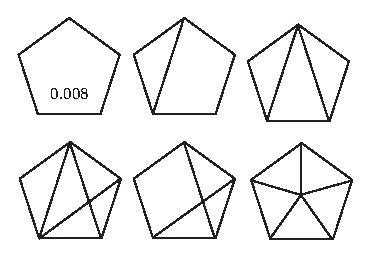
\includegraphics{PS/penthex.eps}
  \caption{Pentagonal Face Refinements}
  \label{fig:penthex}
\end{figure}

\begin{figure}[htb]
  \centering
  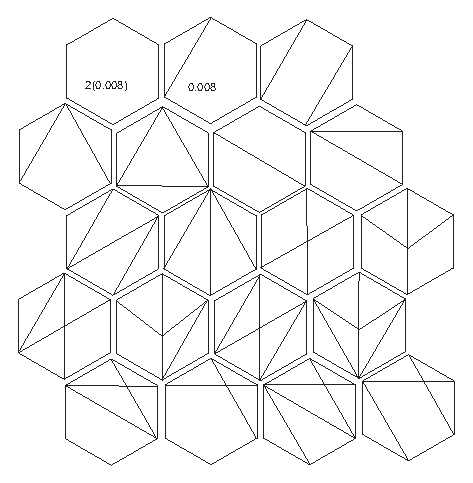
\includegraphics{PS/hexrefine_xxx.eps}
  \caption{Hexagonal Face Refinements.
    The only figures with a penalty are the first two on the top
    row and those on the bottom row.  The first two on the top row
    have penalties $2(0.008)$ and $0.008$.  Those on the bottom
    row have penalties $3\xiG$, $3\xiG$, $\xiG+2\xiV$, and
    $\xiG+2\xiV$.
  }
  \label{fig:hexrefine}
\end{figure}

The conventions for generating the possibilities are different for
the pentagons and hexagons than for the heptagons and octagons. We
describe the pentagons and hexagons first.  We erase all
$3$-unconfined upright diagonals. If there is one loop we leave
the loop in the figure. If there are two loops (so that both
necessarily have context $(n,k)=(4,1)$), we erase one and keep the
other.

The figures are interpreted as follows.  An internal vertex in the
polygon represents an upright diagonal.  Edges from that vertex are
in $1$-$1$ correspondence with the anchors around that upright
diagonal.  Edges between nonadjacent vertices of the polygon
represent the diagonals of flat quarters.  We draw all edges from an
upright diagonal to its anchors, and all edges of length
$[2t_0,2\sqrt2]$ that are not masked by upright quarters. Since the
only remaining upright quarters belong to loops, the four simplices
around a loop are anchored simplices and the edge opposite the
diagonal has length at most $3.2$.

Various inequalities in the inequality archive have been designed
for subregions of pentagons. Additional inequalities have been
designed for subregions in hexagonal regions.  Thus, we are able
to obtain greatly improved linear programming bounds when we break
each pentagonal region into various cases, according to the list
of Figures~\ref{fig:penthex} and \ref{fig:hexrefine}.

\section{Hept and Oct Branching}

When the figure is a heptagon or octagon, we proceed differently.
We erase all $3$-unconfined upright diagonals and all loops
(either context $(n,k)=(4,1)$ or $(4,2)$) and draw only  the flat
quarters.  An undrawn diagonal of the polygon has length at least
$2t_0$.  Overall, in these cases much less internal structure is
represented.

\begin{figure}[htb]
  \centering
  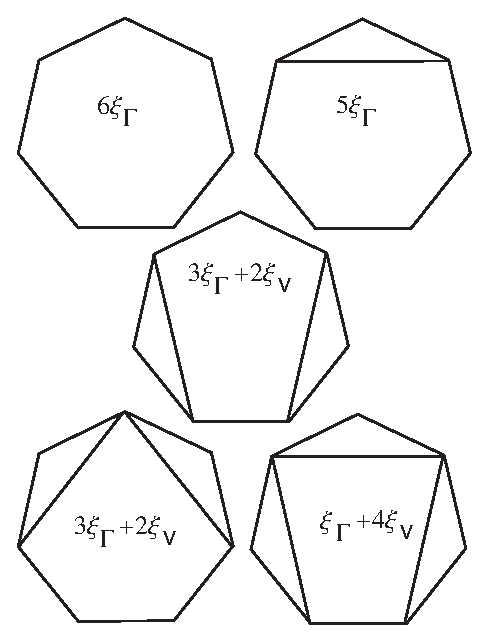
\includegraphics{PS/heptrefine.eps}
  \caption{Hept Face Refinements}
  \label{fig:heprefine}
\end{figure}

\begin{figure}[htb]
  \centering
  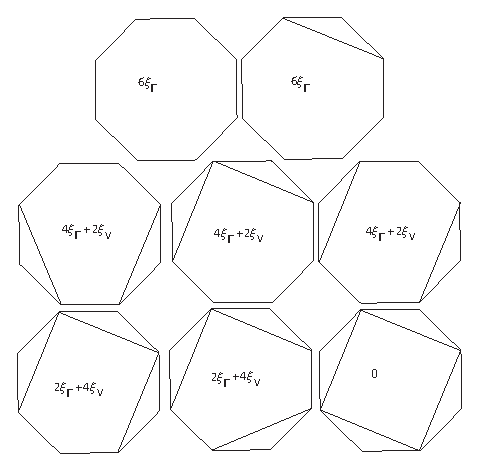
\includegraphics{PS/octrefine.eps}
  \caption{Oct Face Refinements}
  \label{fig:octrefine}
\end{figure}

In the cases where $3$-confined upright diagonals or loops have
been erased, a number indicating a penalty accompanies the
diagram. These penalties are derived in \shortversion{\cite{KC}.}
\longversion{Sections~\ref{sec:penalty} and \ref{sec:penalty1}.}

Define values
    $$
    Z(3,1)=0.00005\quad\text{and }D(3,1)=0.06585.
    $$

Here are some special arguments that are used for heptagons and
octagons.

\subsection{One flat quarter}
Suppose that the standard region breaks into two
subregions: the triangular region of a flat quarter $Q$ and one
other. Let $n=n(R)\in\{7,8\}$. We have the inequality:
    $$
    \sigma_R(D) < (\hat\sigma(Q)-Z(3,1)) + s_{n} +\xiG+2\xiV.
    $$
The penalty term $\xiG+2\xiV$ comes from a possible anchored
simplex masking a flat quarter.   Let $v$ be the central vertex of
the flat quarter $Q$.  Let $\{v_1,v_2\}$ be its diagonal. Masked
flat quarters satisfy restrictive edge constraints.  It follows
from \shortversion{\cite{KC}}
\longversion{Section~\ref{sec:some-flat}} that we have one of the
following three possibilities:
    \begin{enumerate}
    \item $y[v] \ge 2.2$,
    \item $e[v_1,v_2] \ge2.7$,
    \item $\sigma_R(D) < (\hat\sigma(Q)-Z(3,1)) + s_{n(R)}.$
    \end{enumerate}

\subsection{Two flat quarters}
We proceed similarly if the standard region $R$ breaks
into three subregions: two regions $R_1$ and $R_2$ cut out by flat
quarters $Q_1$, $Q_2$ and one other region made from what remains.
Write $\hat\sigma_1$ for $\hat\sigma(Q_1)$, and so forth.  It
follows from \shortversion{\cite{KC}}
\longversion{Section~\ref{sec:some-flat}} that we have one of the
following three possibilities:
    \begin{enumerate}
    \item The height of a central vertex is at least $2.2$.
    \item The diagonal of a flat quarter is at least $2.7$.
    \item
        $$
        \begin{array}{lll}
        \sigma_R(D) &< (\hat\sigma_1-Z(3,1)) +
            (\hat\sigma_2-Z(3,1))+ s_{n(R)},\\
        \tau_R(D)
        &>(\hat\tau_1-D(3,1))+(\hat\tau_2-D(3,1))+t_{n(R)}.
        \end{array}
        $$
    \end{enumerate}


With heptagons, it is helpful on occasion to use an upper bound on the
penalty of $3\xiG = 0.04683$. This bound holds if neither flat quarter
is masked by a loop. For this, it suffices to show that first two of the
given three cases do not hold.

%\subsubsection{Octagon Branching}.

If there is a loop of context $(n,k)=(4,2)$, we have the upper
bounds of Lemma~\ref{lemma:loop:bis}.  If, on the other hand,
there is no loop of context $(n,k)=(4,2)$, then we have the upper
bound
    $$
    \sigma_R(D)\le
    (\hat\sigma(Q_1)-Z(3,1)) +
    (\hat\sigma(Q_2)-Z(3,1)) + s_{n(R)} + 2(\xiG+2\xiV),
    $$
where $n(R)\in\{7,8\}$.


\section{Branching on Upright Diagonals} %subsection
\label{sec:4.12}

We divide the upright simplices into two domains depending on the
height of the upright diagonal, using $|v|=2.696$ as the dividing
point. We break the upright diagonals (of unerased quarters in the
$Q$-system) into cases:
    \begin{enumerate}
    \item The upright diagonal has height at most $2.696$.
    \item The upright diagonal $\{0,v\}$ has height at least $2.696$,
        and some anchor $w$ along the flat quarter satisfies
        $|w|\ge 2.45$ or $|v-w|\ge2.45$.  (There is a separate
        case here for each anchor $w$.)
    \item The upright diagonal $\{0,v\}$ has height at least
    $2.696$,
        and every anchor $w$ along the flat quarter satisfies
        $|w|\le 2.45$ and $|v-w|\le2.45$.
    \end{enumerate}
Many inequalities have been specially designed to hold on these smaller
domains.  They are included into the linear programming problems as
appropriate.

When all the upright quarters can be erased, then the case for
upright quarters follows from some other case without the upright
quarters.  An upright quarter can be erased in the following
situations.  If the upright quarter $Q$ has compression type (in
the sense of Definition~\ref{def:sigma}) and the diagonal has
height at least $2.696$,
then\footnote{\calc{214637273}. %Here $\sigma=\nu_\Gamma$.
}
    $$\sigma(Q)<\svor_0(Q)$$
%(Calculations~\ref{x-calc:AA10}).
(If there are masked flat quarters, they become scored by
$\hat\sigma$.) If an upright quarter has Voronoi type and the
anchors $w$ satisfy $|w|\le 2.45$ and $|v-w|\le2.45$, then the
quarter can be erased\footnote{\calc{378432183}.  %Here $\sigma=\nu$.
}
    $$\sigma(Q)<\svor_0(Q)$$
In general, we only have the weaker
inequality\footnote{\calc{310679005}.  %Here $\sigma=\nu$.
}
%(Inequality~\ref{x-calc:AA11})
    $$\sigma(Q)< \svor_0(Q)+0.003521.$$


%\section{Branching on Upright Quarters} %section
%\label{sec:6}

In a pentagon or hexagon, consider an upright diagonal with three
upright quarters, that is, context $(n,k)=(4,1)$. If the upright
diagonal has height at most $2.696$, and if an upright quarter
shares both faces along the upright diagonal with other upright
quarters, then we may assume that the upright quarter has
compression type. For otherwise, there is a face of circumradius
at least $\sqrt2$, and
hence two upright quarters of Voronoi type.  The inequality % where is this?
    \begin{equation} \octavor <
    \octavor_0 - 0.008,
    \label{eqn:6.1}
    \end{equation}
if $y_1\in[2t_0,2.696]$, and $\eta_{126}\ge\sqrt2$ shows that the
upright quarters can be erased without penalty because
    $$\xiG -0.008-0.008 <0.$$
If erased, the case is treated as part of a different case.

This allows the inequalities\footnote{See, for example,
\calc{867513567-*}} to be used that relate specifically to upright
quarters of compression type.
% Appendix \ref{app:nugamma1} and \ref{app:nugamma}
Furthermore, it can often be concluded that all three upright
quarters have compression type. For this, we use various
inequalities in the archive
    %%\ref{app:471} and \ref{app:455}}
which can often be used to show that if the anchored simplex has a
face of circumradius at least $\sqrt2$, then the linear
programming bound on $\sigma(D)$ is less than $8\,\pt$.



\section{Branching on Flat Quarters}

We make a few general remarks about flat quarters.



\begin{remark}
Information about the internal structure of an exceptional face
gives improvements to the constants $1.4\,\pt$ and $1.5\,\pt$ of
Property \ref{definition:admissible:excess} in the definition of
admissible weight assignments. (The bounds remain fixed at
$1.4\,\pt$ and $1.5\,\pt$, but these arguments allow us to specify
more precisely which simplices contribute to these bounds.) These
constants contribute to the bound on $\tau(D)$ through the
admissible weight assignment. Assume that at the vertex $v$ there
are four quasi-regular tetrahedra and an exceptional face, and
that the exceptional face has a flat quarter with central vertex
$v$. The calculations of Section \ref{sec:tri34} show that the
union $F$ of the four quasi-regular tetrahedra and exceptional
region give $\tau_F(D)\ge 1.5\,\pt$. If there is no flat quarter
with central vertex $v$, then the union $F$ of four quasi-regular
tetrahedra along $\{0,v\}$ give $\tau_F(D)\ge 1.5\,\pt$. We can make
similar improvements when $tri(v)=3$.
\end{remark}

\begin{remark} There are a few  other interval-based inequalities that are
used in particular cases. The inequalities
    $y_1\le 2.2, y_4\le2.7, \eta_{234},\eta_{456}\le\sqrt2$
imply that the flat quarter has compression type (see
Section~\ref{sec:rules}). The circumradius is not a
linear-programming variable, so its upper bound must be deduced
from edge-length information.
\end{remark}

If all three corners of a flat quarter have height at most 2.14,
and if the diagonal has length less than $2.77$, then the
circumradius of the face containing the origin and diagonal is at
most $\eta(2.14,2.14,2.77)<\sqrt2$.  This allows us to branch
combine into three cases.
\begin{lemma}
    Let $Q$ be a flat quarter whose corners $v_i$ have height at most $2.14$ and
    whose diagonal is at most $2.77$.  Then one of the following is true.
        \begin{enumerate}
    \item $\sigma(Q)=\Gamma(Q)$.
    \item The diagonal has length $\le2.7$, $\eta(y_4,y_5,y_6)\ge\sqrt2$,
        and $\sigma(Q)\le \svor_0(Q)$.
    \item The diagonal has length $\ge2.7$ and $\sigma(Q)\le\svor_0(Q)$.
    \end{enumerate}
\end{lemma}

\begin{proof} Case 1 holds when $Q$ is a quarter of compression
type in the $Q$-system.  If $Q$ is in the $Q$-system but is not of
compression type, then $\eta(y_4,y_5,y_6)\ge\sqrt2$ and
$\sigma(Q)\le \svor_0(Q)$.  If $Q$ is not in the $Q$-system, then
$\svor_0(Q)$ is an upper bound \shortversion{\cite{KC}.}
\longversion{Lemma~\ref{lemma:hatsigma}.} If $Q$ is not in the
$Q$-system, then its diagonal has length at least $2.7$, or the
central vertex has height at most $2.2$ (see
Lemma~\ref{lemma:2.7}.) In this case, we use the upper bound
$\svor_0(Q)$.
\end{proof}

Various inequalities in the archive have designed specifically for
each of these three cases.  Thus, whenever the hypotheses of the
lemma are met, we are able to improve on the linear programming
bounds by breaking into these three cases.
%We use the specially tailored Inequalities \ref {app:A.7.1} and
%\ref {app:A.7.2}.

\section{Branching on Simplices that are not Quarters}

\begin{lemma}
Suppose that  a triangular subregion comes from a simplex $S$ with
one vertex at the origin and three other vertices of height at
most $2t_0$.  Suppose that the edge lengths of the fourth, fifth,
and sixth edges satisfy $y_5,y_6\in[2t_0,2\sqrt2]$,
$y_4\in[2,2t_0]$. Suppose that $\min(y_5,y_6)\le2.77$. Then one of
the following is true.
    \begin{enumerate}
    \item  The edges have lengths $y_5,y_6\in[2t_0,2.77]$,
    $\eta_{456}\ge\sqrt2$, and $\sigma(S) \le \svor_0(S)$.
    \item
    $y_5,y_6\in[2t_0,2.77]$, and $\sigma(S) \le \svor(S)$
     (the analytic Voronoi function).
    \item An edge (say $y_6$)
    has length $y_6\ge2.77$ and $\sigma(S) \le \svor_0(S)$.
    \end{enumerate}
\end{lemma}

\begin{proof} If we ignore the statements about $\sigma$, then the
conditions in the Lemma concerning edge-length are exhaustive.
The bounds on $\sigma$ in each case are given by
\shortversion{\cite{KC}.}
\longversion{Section~\ref{sec:separation}.}
\end{proof}

There are linear programming inequalities that are tailored to
each case.

%We use the specially tailored Inequalities \ref{app:17}.

%If there is an enclosed vertex of height at most $\sqrt2$, then we can
%use Inequalities \ref{app:A.7.4}.


\longversion{\section{Branching on Quadrilateral subregions}}

\longversion{One of the inequalities of
%\ref{app:471}
holds for a quadrilateral subregion, if certain conditions are
satisfied.  One of the conditions is $y_4\in[2\sqrt2,3.0]$, where
$y_4$ is a diagonal of the subregion. Since this diagonal is not
one of the linear programming variables, these bounds cannot be
verified directly from the linear program.  Instead we use an
inequality
%\ref{ineq:1.678}
which relates the desired bound $y_4\le3$ to the linear
programming variables $\alpha[v,F]$, $y_2$, $y_3$, $y_5$, and
$y_6$.}
